% qjrms4doc.tex V1.10, 4 October 2013

\documentclass[times]{qjrms4}
\usepackage[colorlinks,bookmarksopen,bookmarksnumbered,citecolor=red,urlcolor=red]{hyperref}
\usepackage{moreverb}

%\def\volumeyear{2013}
\def\volumenumber{00}

\begin{document}

\runningheads{A.~R.~Herrington and K.~A.~Reed}{CAM resolution sensitivity}

\title{Parameterized convection, grid-scale clouds and resolution sensitivity in the Community Atmosphere Model}

\author{Adam R. Herrington\corrauth, Kevin A. Reed}
\address{School of Marine and Atmospheric Sciences, Stony Brook University, Stony Brook, NY 11794}

\corraddr{\url{adam.herrington@stonybrook.edu}}

\begin{abstract}
This paper describes...
\end{abstract}

\keywords{Climate models, physical parameterizations, physics-dynamics coupling}

\maketitle

\section{Introduction}

An increasing number of Atmospheric General Circulation Models (AGCMs) are being developed to maximize efficiency on massively parallel systems, permitting regionally-refined high-resolution, or even globally high-resolution weather ($\Delta x = 5$ km and less) and climate ($\Delta x = 50$ km and less) simulations \citep{MPASatm,Z2014QJRMS,HETAL2016JCLIM,DCMIP16,LetAl2018JAMES}. These models are built using unstructured meshes that while allows for substantial grid flexibility, require physical parameterizations ({\em{physics}}) that behave consistently as the truncation scale of the model changes with different grid resolutions, referred to as scale-aware physics. The most common approach towards developing scale-aware physics is through the lens of limited area, large-eddy simulations \citep[e.g.,][]{PC2008JAS,AW2013JAS,SZ2018JCLIM}. Through subsequently filtering large-eddy solutions to lower-resolution grids, a relationship between first- and higher-order moments \citep{G1992JFM} may be understood and ultimately parameterized as a function of grid resolution. While this approach is likely necessary for developing scale-aware physics, it is not sufficient. The equations of motions have inherent scale dependencies, with the properties of dynamical modes a function of native grid resolution \citep{O1981JAS,WETAL1997MWR,PG2006JAS,JR2016QJRMS}. Scale-aware physics should also recognize these native grid dependencies.

The sensitivity of the Community Atmosphere Model \citep[CAM;][]{CAM5}, and its predecessor, the Community Climate Model (CCM) to resolution ({\em{resolution}} refers to {\em{horizontal resolution}}, hereafter) is well documented through convergence studies \citep{KW1991JGR,WETAL1995CD,W2008TELLUS,RETAL2013JCLIM,ZetAl2014JCb,HR2017JCLIM}. Despite thirty years of continual model development, there are robust sensitivities to resolution that have persisted in all versions of the model. This study argues that a unifying cause, the inherent scale sensitivities of the underlying dynamical equations, can explain the robust responses to resolution that occur in CAM/CCM, {\color{red}{since it is difficult to conceive that inevitable responses to native grid resolution could be ignored in the pursuit of scale-aware physics.}}

In CAM/CCM, the atmosphere progressively dries with increasing resolution, seen through a reduction in simulated total precipitable water \citep{KW1991JGR,WETAL1995CD,W2008TELLUS,RETAL2013JCLIM,ZetAl2014JCb,HR2017JCLIM}, which typically, but not always \citep[see][]{WETAL1995CD,ZetAl2014JCb}, coincides with a reduction in cloud cover. \cite{KW1991JGR} and \cite{WETAL1995CD} suggested that the drying of the atmosphere is due to greater magnitude resolved vertical velocities with increasing resolution, with greater subsiding motion increasing the export of dry air from the upper troposphere. This mechanism is consistent with an analysis of moisture budgets in CAM, version 4 \citep[CAM4;][]{CAM4} across multiple resolutions \citep{YETAL2014JCLIM,HR2017JCLIM}.

It is well known that the magnitude of vertical velocities increase with resolution in atmospheric models. While the cause of this sensitivity has been established for large-eddy simulations \citep[see][and references therein]{J2017JAMES}, only recently has the vertical velocity field in AGCMs and their sensitivity to resolution received attention \citep{DETALA2016ACP,OETAL2016JAMES}, albeit with conflicting explanations \citep{RETAL2016CD,HR2018JAMES}. To generalize the relationship between vertical velocity and resolution, let $\alpha$ refer to the ratio of $W_0$, the vertical velocity scale of some reference grid spacing $\Delta x_0$, to $W$, the vertical velocity scale of any $\Delta x$. A power law for $\alpha$ in $\Delta x$ is then,
\begin{equation}
\alpha = \frac{W_0}{W} = \left( \frac{\Delta x_0}{\Delta x} \right)^n, \label{eq:alpha}
\end{equation}
where $n$ is the power law exponent. 

\cite{RETAL2016CD} derive an estimate $n= b-1$ by combining a scale analysis of the continuity equation with a power law representation $\Delta x^{2b}$ of the second-order structure function of the horizontal wind. Strictly speaking, $\Delta x$ here refers to the distance between two points for which the velocity increment is computed in the structure function, but with this distance set to the model grid-spacing. Observations indicate that $b=\frac{1}{3}$ for scales less than about $1000$ km \citep{CETAL1999JGR}, which according to the Weiner–Khinchin theorem $- \left( 2b+1 \right) = -\frac{5}{3}$ is equal to the slope of the kinetic energy spectrum for mesoscale motions \citep{NG1985JAS}. \cite{RETAL2016CD} argue that the $-\frac{5}{3}$ slope is common in both observations and models, and provides an emergent constraint for $n= -\frac{2}{3}$.

In large-eddy simulations, the sensitivity of vertical velocities to resolution is adequately explained by a scale analysis of the dynamical equations \citep{WETAL1997MWR,PG2006JAS,JR2016QJRMS}. For hydrostatic scales relevant to AGCMs, a scale analysis of the Poisson equation gives $W \propto D^{-1}$, where $D$ is the horizontal scale of a buoyancy perturbation driving vertical motion \citep{HR2018JAMES}. In CAM aqua-planet simulations, the largest source of buoyancy is from grid-scale cloud formation, whose horizontal extents are set by the effective resolution of the model (i.e., some multiple of $\Delta x$), indicating $n=-1$ \citep{HR2018JAMES}. \cite{HR2017JCLIM} has shown that the $n=-1$ scaling does not explain the behavior of CAM4 in a convergence experiment, but follow-up studies \citep{HR2018JAMES,HETAL2019JAMES} indicate that the inadequacy of the $n=-1$ scaling is not definitive due to time-truncation errors associated with fixing the physics time-step ($\Delta t_{phys}$) across resolutions in that study.

Another robust response of the CAM/CCM lineage to resolution is an increase in stratiform precipitation rates (i.e., the precipitation from grid-scale clouds), at the expense of parameterized convective precipitation rates. This behavior is summarized in Figure~\ref{fig:cam-history}, which is a bar-graph of the climatological, global mean stratiform and convective precipitation rates in prior CAM/CCM convergence studies. The studies of \cite{KW1991JGR}, \cite{WETAL1995CD} and \cite{W2013QJRMS} indicate that the tendency to reduce $\Delta t_{phys}$ with resolution would by itself reduce the convective precipitation rates, however Figure~\ref{fig:cam-history} (top row) indicates that convergence studies with fixed $\Delta t_{phys}$ still show a reduction in convective precipitation rates with resolution.

\begin{figure}[t]
\begin{center}
\noindent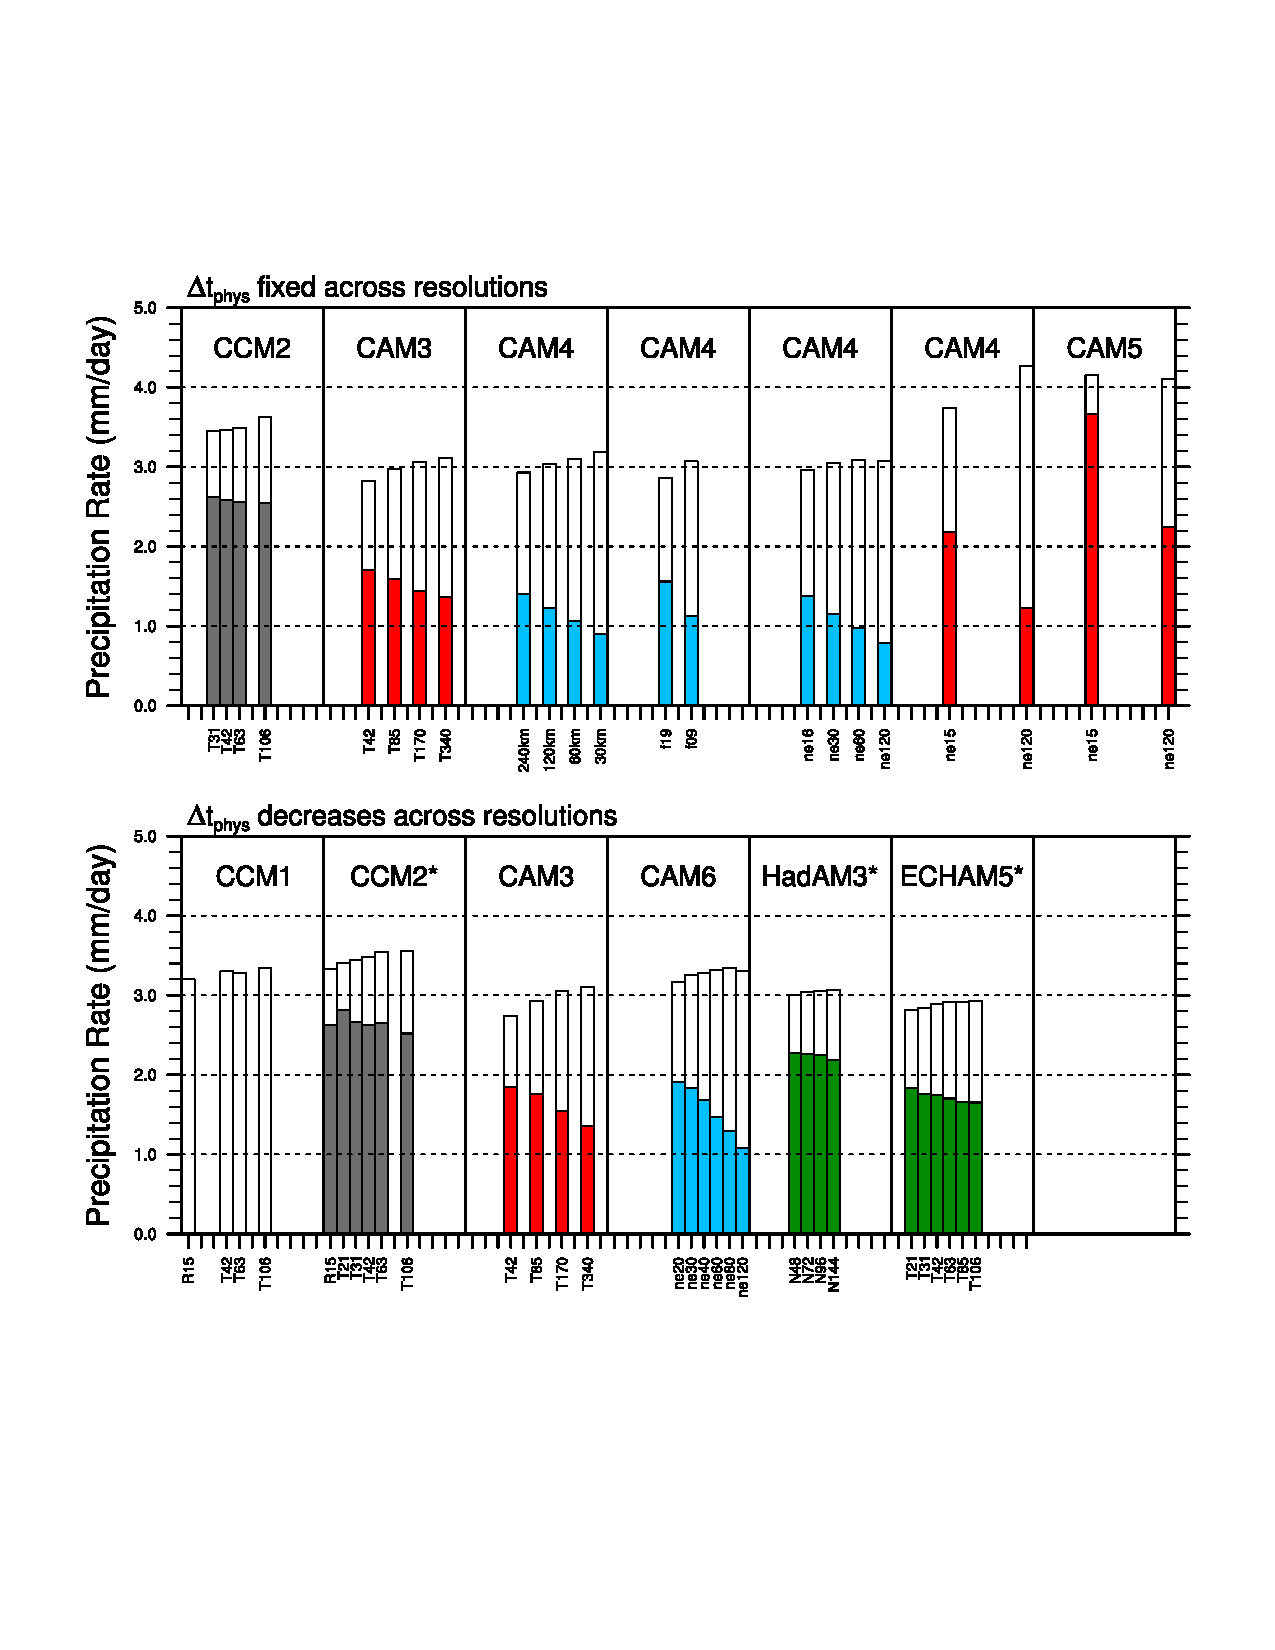
\includegraphics[width=20pc,angle=0]{figs/cam-history.pdf}\\
\end{center}
\caption{Bar-graph of the convective (solid) and grid-scale (white) climatological precipitation rates in prior CAM/CCM convergence studies. Each window contains a single convergence study, with identical x-axis; the approximate grid resolution. Colors indicate the model configuration; January ensemble (black) and aqua-planet configurations with SST profiles $QOBS$ (blue) and $CNTL$ (red) after \cite{NH2000ASL}. Studies included in this figure are \cite{KW1991JGR} (CCM1), \cite{WETAL1995CD} (CCM2), \cite{W2008TELLUS} (CAM3), \cite{RETAL2013JCLIM,ZetAl2014JCb,HR2017JCLIM} (CAM4), \cite{ZetAl2014JCb} (CAM5) and this study (CAM6). CCM2* refers to the modified parameter experiment of \cite{WETAL1995CD}, where parameters vary with resolution to reduce the dependence of cloud fraction on resolution.}
\label{fig:cam-history}
\end{figure}

In this study, a convergence experiment using CAM, version 6 (CAM6; \url{https://ncar.github.io/CAM/doc/build/html/users_guide/index.html}) is carried out and analyzed in detail. It is shown that the resolution sensitivity of vertical velocities are well described with $n=-1$ in equation~\eqref{eq:alpha}, provided $\Delta t_{phys}$ is defined in a way that avoids large truncation errors across resolutions. The reduction in convective precipitation rates with resolution in CAM6 is shown to result from the greater magnitude subsiding motion, creating a more stable atmosphere in which the criterion for parameterized convection occurs less often. The feedback of the resolved vertical motion on the physics indicates that the root cause of resolution sensitivity in CAM arises from the sensitivity of resolved dynamical modes to native grid resolution. Section 2 describes CAM6 and details the convergence experiment. Section 3 contains a thorough analysis of the CAM6 simulations and Section 4 provides some discussion and conclusions.

\section{Methods}

\subsection{Dynamical Core}

This study uses the spectral-element dynamical core option of Community Atmosphere Model \citep[CAM-SE;][]{DetAl2012IJHPCA}, coupled with a mass conserving, semi-Lagrangian advection method for accelerated multi-tracer transport \citep[CSLAM;][]{LTOUNGK2017MWR}, and dry-mass vertical coordinate with comprehensive treatment of moisture and energy \citep{LetAl2018JAMES}. The dry dynamics are solved using the high-order, momentum, mass and energy conserving spectral element method \citep{TF2010JCP}, with the elements defined by a cubed-sphere grid. The notation for the horizontal grid resolution is an `$ne$' followed by the number of elements making up an edge of one cubed-sphere face, e.g., $ne30$. Hyper-viscous $\nabla^{4}$ explicit numerical dissipation is applied to temperature, dry pressure thickness, rotational and divergent winds. CSLAM tracer transport uses a finite volume grid constructed from the cubed-sphere of elements, and contains the same degrees of freedom as the dry dynamics.

\subsection{Physical Parameterizations}

The physics are evaluated on the finite-volume CSLAM grid, and the tendencies mapped back to the spectral element grid. The coupled system, referred to as CAM-SE-CSLAM, conserves energy, mass and preserves linear correlations between two reactive species to within machine precision \citep{HL2018MWR}. A coarser physics grid, containing $\frac{5}{9}$ fewer degrees of freedom than the dynamical core grid is also available as part of the CAM-SE-CSLAM package \citep{HETAL2019JAMES}. This lower-resolution physics grid is used in this study, but only as a member of a perturbed parameter ensemble and not in the default convergence experiment. The dynamics time-step is subcycled within a longer physics time-step $\Delta t_{phys}$, and the temperature and momentum increments from the physics are divided by the number of subcycles and added to the dynamical core at the beginning of each subcycle. The full moisture increment from the physics is applied only at the start of the first subcycle to conserve tracer mass \citep[$ftype=2$ option in][]{LetAl2018JAMES}.

The simulations use the CAM6 physics package. The Cloud Layers Unified by Binormals \citep[CLUBB][]{GETAL2002JAS,BOG2013JCLIM} is an assumed probability distribution function (PDF) high-order closure model that handles shallow convection, planetary boundary layer mixing and cloud macrophysics. The macrophyiscs are coupled with a two-moment bulk cloud microphysics scheme with prognostic precipitation \citep{MG2}, and microphysics are coupled with a three mode Modular Aerosol Model \citep{MAM}. The combined macrophysics/microphysics routines generate grid-scale clouds with stratiform precipitation. Deep convection is parameterized using a quasi-equilibrium mass flux scheme \citep{ZM1995AO} and a dilute form of the convective available potential energy (CAPE) is computed and used as the convective trigger (convection occurs if dilute CAPE $\geq 70$ J/kg), and for closing the mass fluxes in the cloud ensemble \citep{NRJ2008JC}. The deep convection scheme also parameterizes convective momentum transport \citep{RR2008JC}.

\subsection{Experimental Design}
 
The convergence experiment is performed in an aqua-planet configuration \citep{NH2000ASL,MWO2016JAMES}, an all ocean planet with fixed, zonally symmetric sea surface temperatures modeled after present day Earth \citep[$QOBS$ in][]{NH2000ASL}. The aqua-planets are in a perpetual equinox, and aerosols are largely absent from the simulations. Each simulation is ran for one simulated year. Six different horizontal grids are used in this study, which are provided in Table~\ref{tbl:table1}. The horizontal hyper-viscosity operators $\nu$ vary with resolution after \cite{HETAL2019JAMES}, also provided in Table~\ref{tbl:table1}. The values of $\nu$ are a factor 2.5 greater for divergence damping and are not shown. $\Delta t_{phys}$ is chosen to scale with resolution, in proportion to the grid spacing,
\begin{equation}
\Delta t_{phys} = \Delta t_{phys,0} \times \frac{n_{e,0}}{n_e}~s,\label{eq:dt-scale}
\end{equation}
where $\Delta t_{phys,0}$ is taken to be the standard $1800 s$ used in CAM-SE-CSLAM at the standard resolution, $n_{e,0} = ne30$ (equivalent to an average equatorial grid spacing $\Delta x = 111.2$km). This scaling was chosen to avoid large time-truncation errors in a rising moist bubble test \citep[Appendix A in][]{HETAL2019JAMES}, and it is understood that this choice of $\Delta t_{phys}$ will likely lead to greater resolution sensitivity \citep{W2008TELLUS}. The convective time-scale in the deep convection scheme is fixed at 3600 s in all simulations.
 
\section{Results}

 \begin{table}
 \caption{Experimental design and global means.}
 \centering
 \scriptsize
 \begin{tabular}{lcccccc}
   \hline
   Variable & $ne20$ & $ne30$ & $ne40$ & $ne60$ & $ne80$ & $ne120$ \\ 
   \hline
   $\Delta x$ (km) & 166.8 & 111.2 & 83.4 & 55.6 & 41.7 & 27.8 \\
   $\nu$ ($m^4/s$) & $1.5 \times 10^{15}$ & $4.0 \times 10^{14}$ & $1.5 \times 10^{14}$ & $4.0 \times 10^{13}$  & $1.5 \times 10^{13}$ & $4.0 \times 10^{12}$\\
    $\Delta t_{phys}$ (s) & 2700 & 1800 & 1350 & 900 & 675 & 450 \\
   Total Cloud Fraction & 0.844 & 0.835 & 0.824 & 0.810 & 0.804 & 0.800 \\ 
   Total Precipitable Water (mm) & 23.31& 23.01 & 22.62 & 22.25 & 21.93 & 21.72 \\
   Convective Precipitation (mm/day) & 1.91 & 1.83 & 1.68 & 1.47 & 1.29 & 1.08 \\
   Stratiform Precipitation (mm/day) & 1.26 & 1.42 & 1.60 & 1.85 & 2.05 & 2.22 \\      
 \hline
 \end{tabular}
 \label{tbl:table1}
 \end{table}

Table~\ref{tbl:table1} provides globally averaged, climatological (omitting the first month) metrics for the CAM6 simulations which are typically published in CAM/CCM convergence studies. Total precipitable water, total cloud fraction and deep convective precipitation rate decreases, while stratiform precipitation increases, monotonically with resolution. Resolution sensitivity in CAM6 is similar to all prior versions of the model. 

\subsection{Vertical Velocities and Resolution}

\begin{figure}[t]
\begin{center}
\noindent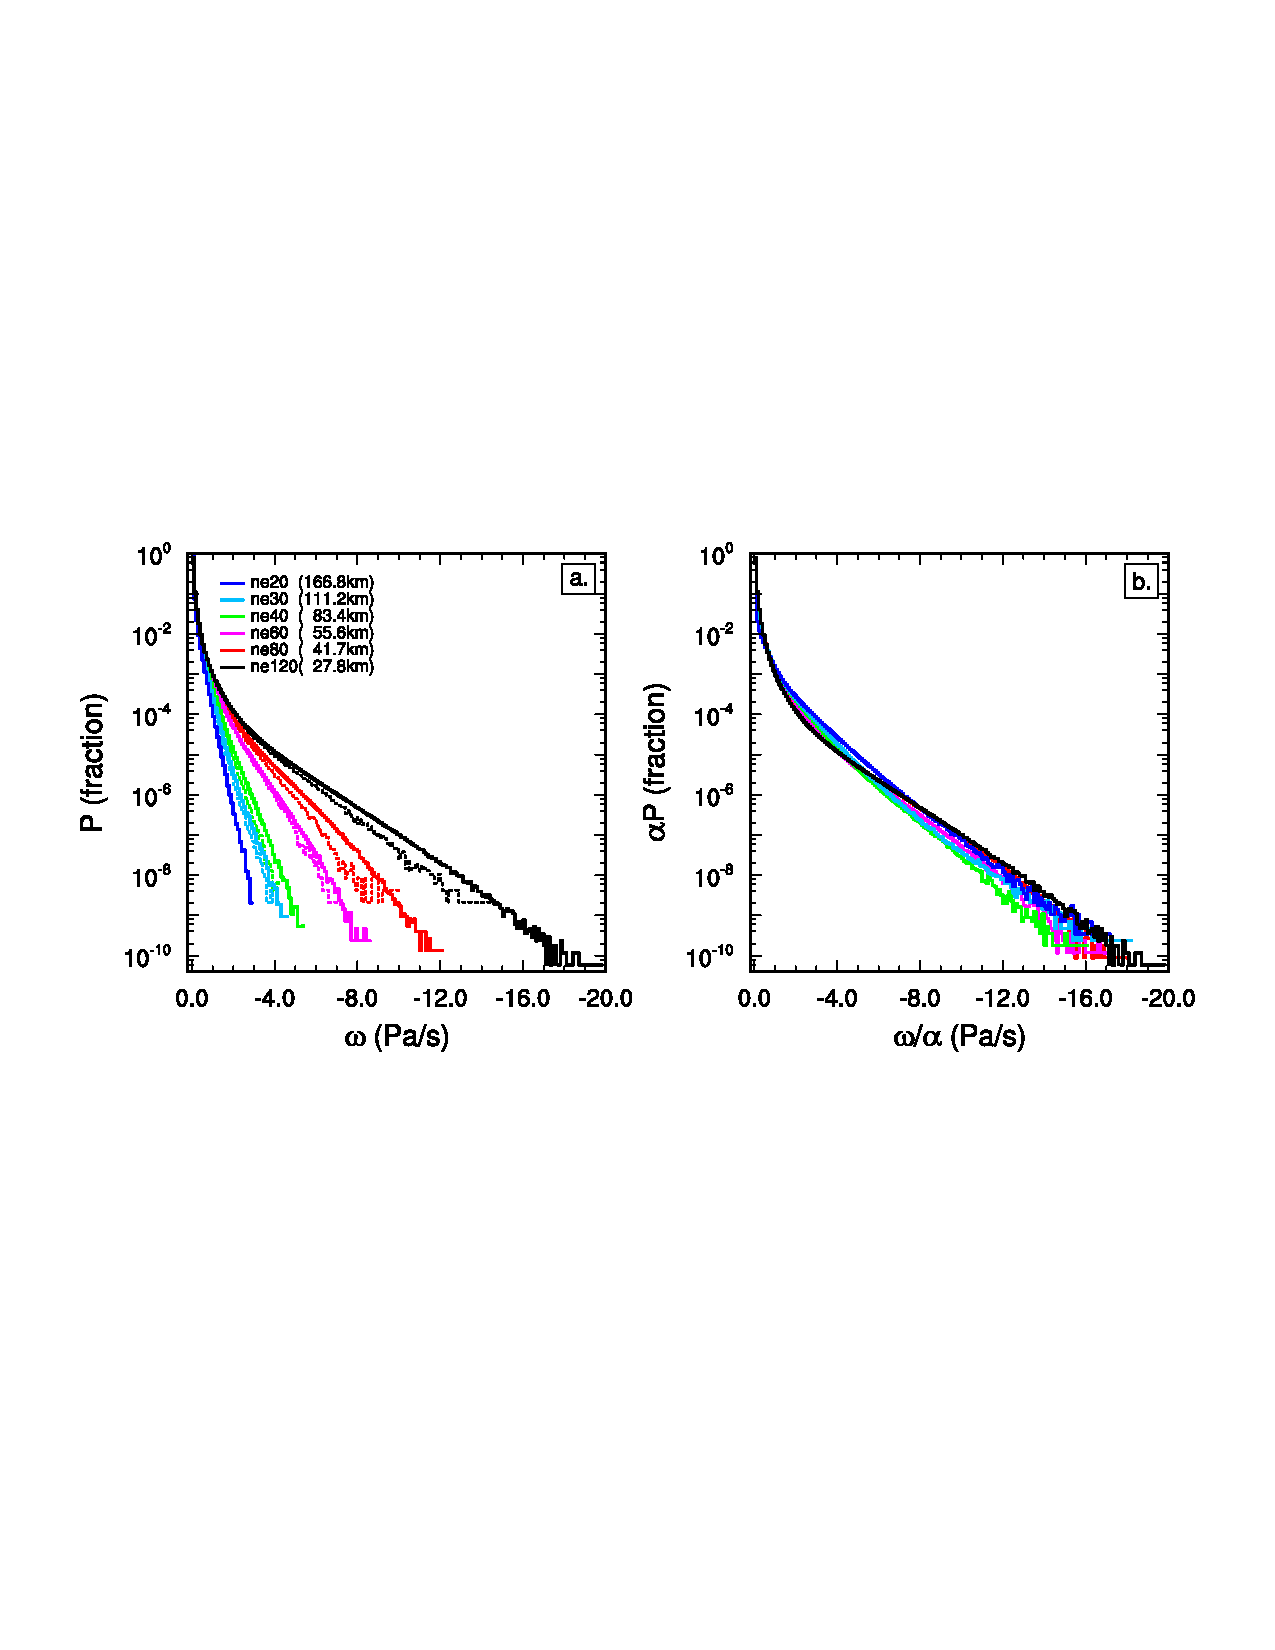
\includegraphics[width=20pc,angle=0]{figs/temp_2pdf.pdf}\\
\end{center}
\caption{Probability density distribution of the upward vertical pressure velocities $\omega$ computed everywhere in the model from 1 year of 6-hourly data (a) raw values (solid) and values remapped to the $ne20$ grid (dotted), (b) values scaled to the $ne120$ resolution.}
\label{fig:2pdf}
\end{figure}

The PDF of negative, or upward vertical pressure velocities $\omega$ in the aqua-planets is shown in Figure~\ref{fig:2pdf}a. The magnitude of upward $\omega$ increases monotonicaly with resolution, with positive, or downward $\omega$ behaving similarly (not shown). This monotonic increase in the magnitude of $\omega$ is evident even after remapping all the model output to a common grid ($ne20$; dotted curves Figure~\ref{fig:2pdf}a).

The PDF's may be scaled to the highest-resolution resolution grid through $P(\omega)_s = \alpha P (\omega / \alpha)$, where $\alpha$ is the scale factor from equation~\ref{eq:alpha}, and setting $\Delta x_0$ to the $ne120$ grid-spacing. Figure~\ref{fig:2pdf}b shows the scaled PDFs using $n=-1$ in equation~\ref{eq:alpha}. The scaled PDF's all collapse onto the high-resolution reference, indicating the a power-law with $n=-1$ explains to first-order the variation in vertical velocity with resolution in the aqua-planet simulations. 

Changes to the vertical velocity field can be further understood through decomposing the mass weighted vertical mean $\omega$ into upward and downward components,
\begin{equation}
\langle \omega \rangle =\langle f_{u} \rangle \, \langle \omega_{u} \rangle + \langle f_{d} \rangle \, \langle \omega_{d} \rangle, \label{eq:omega}
\end{equation}
where $\langle f_x \rangle$ and $\langle \omega_x \rangle$ refers to the vertical mass fraction $ \left( \frac{\int dp_x}{\int dp} \right)$ and the $x$ component of the mass weighted vertical mean of $\omega$ $ \left( \frac{\int \omega_x dp_x}{\int dp_x} \right)$, respectively, subscript $u$ refers to upward motion and $d$, downward motion.

The global mean, climatological components $\langle f_{u} \rangle \, \langle \omega_{u} \rangle$ and $\langle f_{d} \rangle \, \langle \omega_{d} \rangle$ are provided in Figure~\ref{fig:4panel}a,b for the aqua-planet simulations. The magnitude of both $\langle f_{u} \rangle \, \langle \omega_{u} \rangle$ and $\langle f_{d} \rangle \, \langle \omega_{d} \rangle$ increase monotonically with resolution, and are both equal and opposite, which is a requirement of mass conservation in the model and a convenient check of the calculation. The individual component $\langle f_{x} \rangle$ varies by only few percent in the simulations, and so the monotonic behavior of $\langle f_{x} \rangle \, \langle \omega_{x} \rangle$ is primarily due to $ \langle \omega_{x} \rangle$ (not shown).

\begin{figure}[t]
\begin{center}
\noindent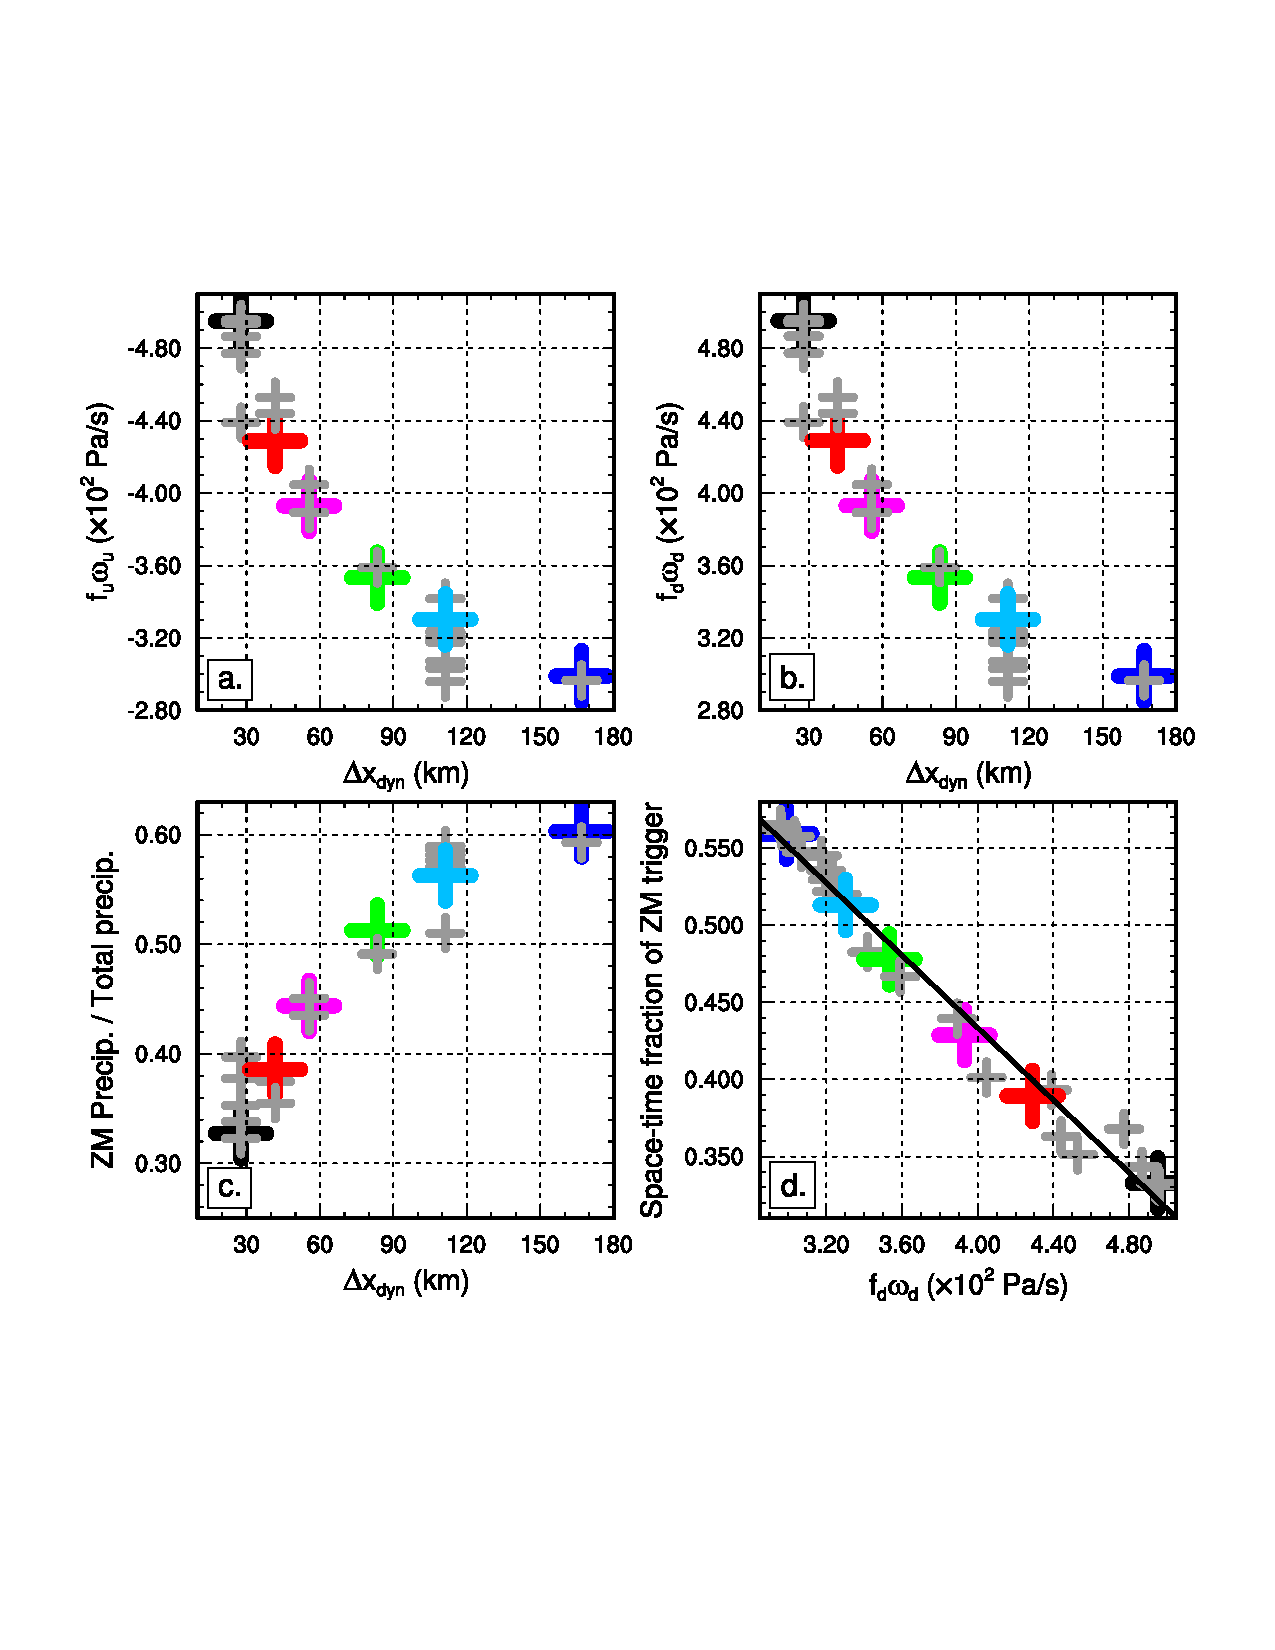
\includegraphics[width=20pc,angle=0]{figs/temp_diags_4panel.pdf}\\
\end{center}
\caption{(a,b,c,e,f,g) Components of the global mean vertical pressure velocity $\overline{\langle \omega \rangle}$ (d) ratio of global mean ZM precipitation rate to the total precipitation rate versus grid spacing $\Delta x$ and (e) scatter plot of $\overline{\langle f_{d} \rangle} \, \overline{\langle \omega_{d} \rangle}$ and FREQZM, and the fitted linear regression which has a Pearson's R-value = 0.99. (a) $\overline{\langle \omega_{u} \rangle}$ (b) $\overline{\langle f_{u} \rangle}$ (c) $\overline{\langle f_{u} \rangle} \, \overline{\langle \omega_{u} \rangle}$ (e) $\overline{\langle \omega_{d} \rangle}$ (f) $ \overline{\langle f_{d} \rangle}$ (g) $\overline{\langle f_{d} \rangle} \, \overline{\langle \omega_{d} \rangle}$. Colors are as in Figure~\ref{fig:2pdf}. Grey crosses are for the perturbed parameter runs.}
\label{fig:4panel}
\end{figure}

\subsection{Convective Precipitation and Vertical Velocities}

The \cite{ZM1995AO} deep convection scheme (referred to as the $ZM$ scheme, hereafter) is modulated by the dilute CAPE calculation, which itself is intertwined with the vertical velocity field \citep{SZ2018JCLIM}. The CAPE budget can be separated into two components \citep{Z2002JGR}; instability due to the thermodynamic state of parcels in the boundary layer and the instability generated through advection of dry static energy and moisture by the environment, i.e., the resolved flow. The latter term is defined as, 
\begin{equation}
-R_d \int_{p_t}^{p_b} \frac{\partial T_{ve}}{\partial t} dlnp \label{eq:cape}
\end{equation}
where $T_{ve}$ is the virtual temperature of the environment, $R_d$ the gas constant for dry air and subscripts $b$ and $t$ refer to the parcel launch level (typically in the boundary layer) and the level of neutral buoyancy, respectively \citep{Z2002JGR}. Equation~\ref{eq:cape} contains a term, the vertical advection of potential energy, which simplifies to $w \frac{\partial gz}{\partial z} = gw$, and directly proportional to the vertical velocity $w$ by the factor $g$, the acceleration of gravity (F. Song, personal communication). In subsiding regions, $w$ is negative and opposes the generation of CAPE through adiabatic warming of the environment.

There is an excellent negative correlation (Pearson's R-value = 0.99) between the global mean, climatological $\langle f_{d} \rangle \, \langle \omega_{d} \rangle$ and a measure of the activity of the ZM scheme in the simulations, $FREQZM$ (Figure~\ref{fig:4panel}c). At any given grid-point and time-step, $FREQZM$ is a binary variable: one if the ZM scheme is active, zero if it is not. Time-mean $FREQZM$ therefore indicates the fraction of the model time that the ZM scheme is triggered, i.e., dilute CAPE exceeds $\geq 70$ J/kg. It is hypothesized that the greater subsiding motion with resolution opposes the generation of dilute CAPE through subsidence warming, reducing the frequency that the ZM scheme is triggered, and leading to the strong negative correlation in Figure~\ref{fig:4panel}c.

\ack This class file was developed by Sunrise Setting Ltd,
Paignton, Devon, UK. Website:\\
\href{http://www.sunrise-setting.co.uk}{\texttt{www.sunrise-setting.co.uk}}

\bibliographystyle{wileyqj}
\bibliography{bib}
\end{document}
